\begingroup
\linespread{1}\selectfont
\definecolor{chfifteencream}{RGB}{255,239,199}
\definecolor{chfifteenblue}{RGB}{173,210,235}
\definecolor{chfifteencoral}{RGB}{255,143,132}
\definecolor{chfifteencyan}{RGB}{0,174,228}
\definecolor{chfifteengreen}{RGB}{75,117,49}
\definecolor{chfifteengold}{RGB}{182,135,26}
\resizebox{0.99\linewidth}{!}{%
\begin{tikzpicture}[x=0.01cm,y=-0.01cm,
  every node/.style={inner sep=0pt,outer sep=0pt},
  chtext/.style={anchor=north west,align=left,font=\fontsize{7.1pt}{8.1pt}\selectfont},
  chtitle/.style={font=\bfseries\fontsize{9.5pt}{10pt}\selectfont},
  chlabel/.style={font=\bfseries\fontsize{7.8pt}{8.2pt}\selectfont}]
\node[anchor=north west] at (0,0) {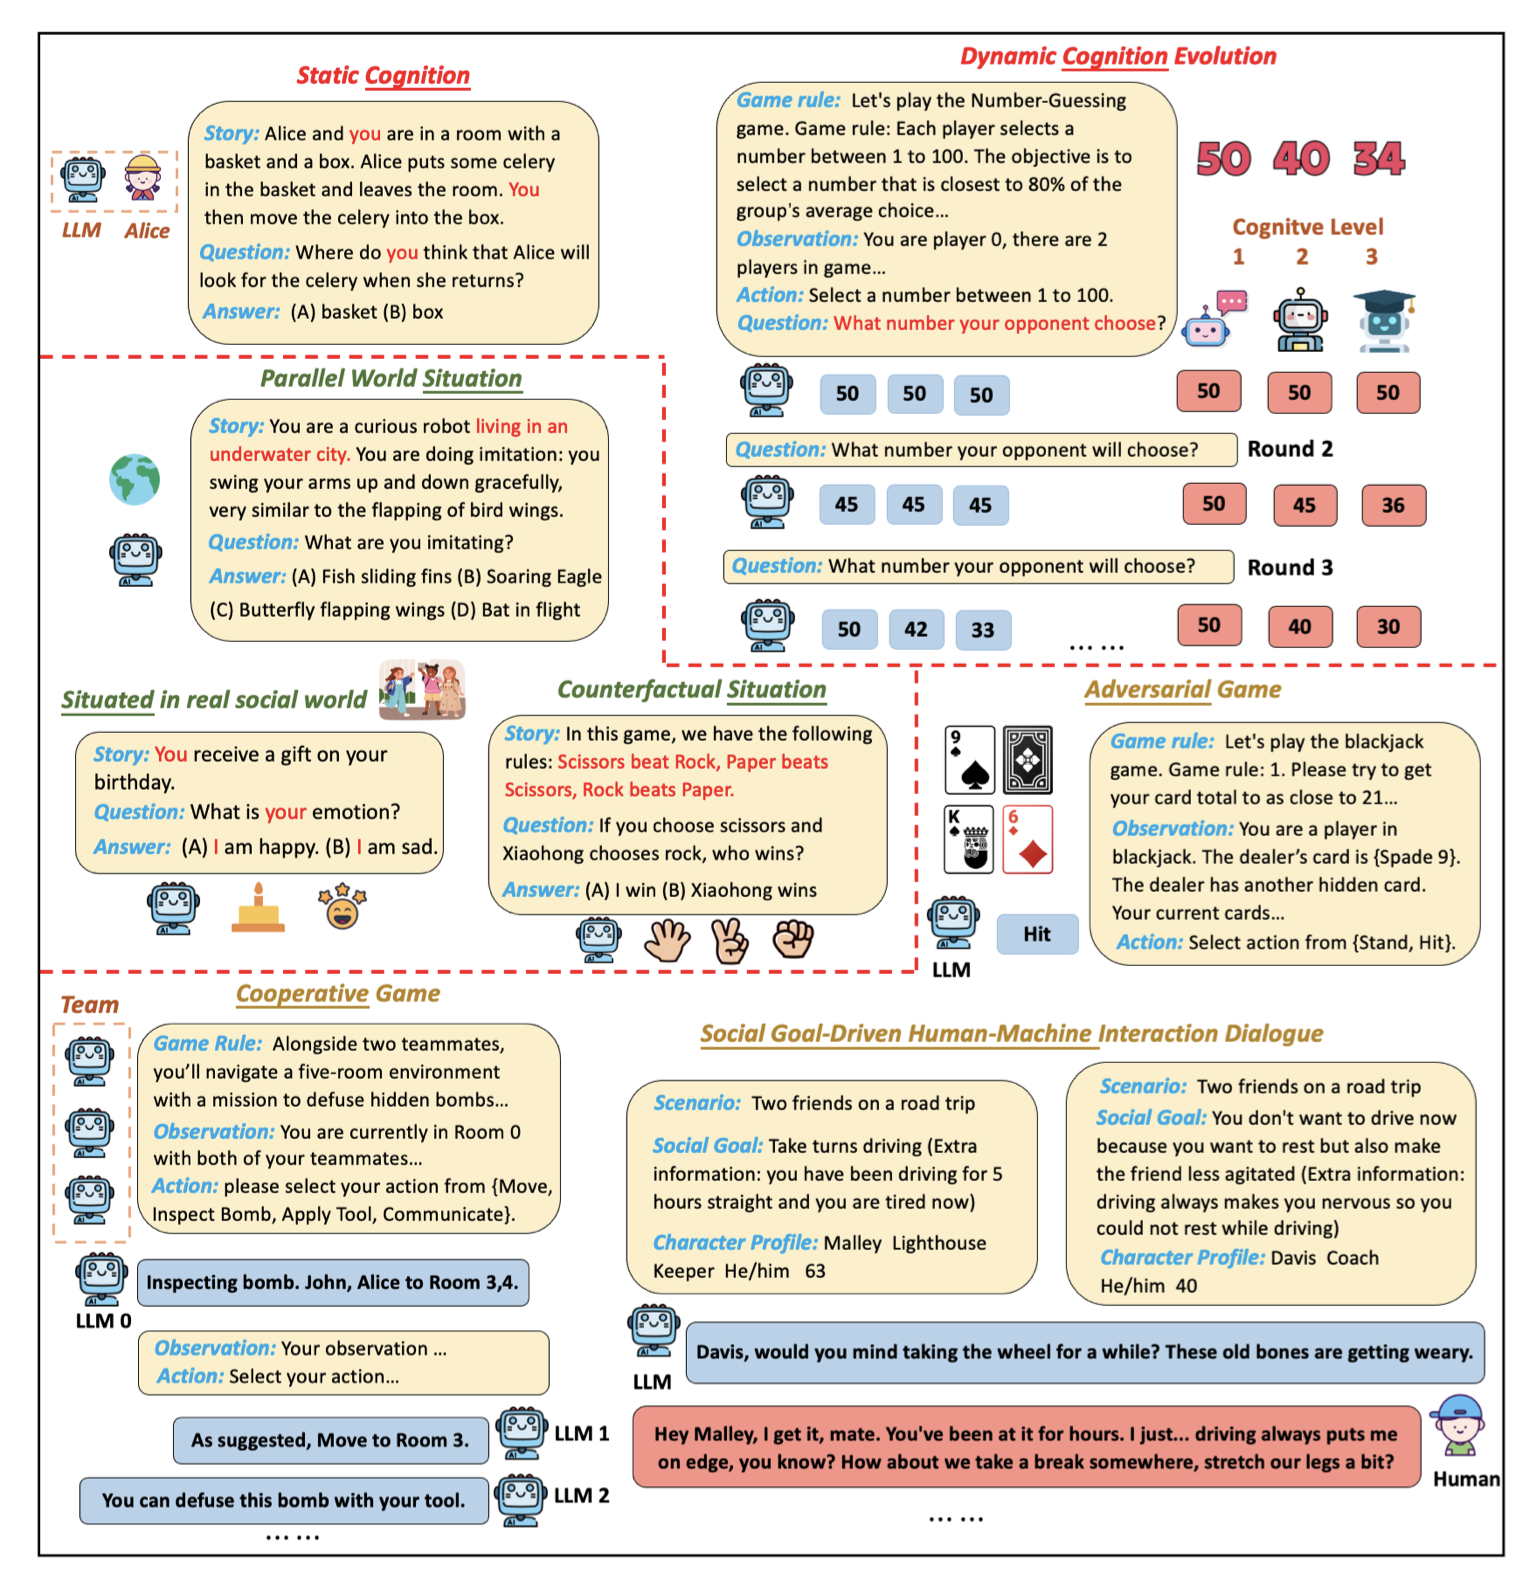
\includegraphics[width=15.36cm]{figures/egosocialarena.png}};
\fill[white] (285,53) rectangle (516,93);
\node[chtitle,text=red] at (396,75) {静态认知};
\fill[white] (187,100) rectangle (600,346);
\draw[fill=chfifteencream,draw=gray,line width=0.4pt,rounded corners=0.42cm] (189,102) rectangle (598,344);
\node[chtext,text width=3.78cm] at (203,122) {
  \textcolor{chfifteencyan}{\bfseries 情境：}Alice 和\textcolor{red}{你}在有篮子和盒子的房间里。Alice 把一些芹菜放进篮子后离开。随后，\textcolor{red}{你}把芹菜移到盒子里。\par
  \textcolor{chfifteencyan}{\bfseries 问题：}\textcolor{red}{你}认为 Alice 回来后会去哪里找芹菜？\par
  \textcolor{chfifteencyan}{\bfseries 答案：}(A) 篮子 (B) 盒子
};
\fill[white] (946,39) rectangle (1290,76);
\node[chtitle,text=red] at (1118,57) {动态认知演化};
\fill[white] (716,81) rectangle (1179,358);
\draw[fill=chfifteencream,draw=gray,line width=0.4pt,rounded corners=0.42cm] (718,83) rectangle (1177,356);
\node[chtext,text width=4.20cm] at (741,107) {
  \textcolor{chfifteencyan}{\bfseries 博弈规则：}来玩猜数游戏。规则：每位参与者选择 1—100 中的一个数。目标是选出最接近全组平均选择值 80\% 的数……\par
  \textcolor{chfifteencyan}{\bfseries 观测：}你是参与者 0，游戏中有 2 名参与者……\par
  \textcolor{chfifteencyan}{\bfseries 动作：}选择 1—100 中的一个数。\par
  \textcolor{chfifteencyan}{\bfseries 问题：}\textcolor{red}{对手选了什么数？}
};
\fill[white] (1225,211) rectangle (1430,242);
\node[chlabel,text=brown] at (1326,227) {认知层级};
\fill[chfifteencream] (734,437) rectangle (1229,463);
\node[chlabel] at (981,450) {\textcolor{chfifteencyan}{问题：}对手将选择什么数？};
\fill[white] (1244,433) rectangle (1350,465);
\node[chlabel] at (1297,450) {第 2 轮};
\fill[chfifteencream] (733,555) rectangle (1226,580);
\node[chlabel] at (980,568) {\textcolor{chfifteencyan}{问题：}对手将选择什么数？};
\fill[white] (1244,550) rectangle (1350,583);
\node[chlabel] at (1297,568) {第 3 轮};
\fill[white] (249,364) rectangle (546,394);
\node[chtitle,text=chfifteengreen] at (398,380) {平行世界情境};
\fill[white] (188,397) rectangle (611,642);
\draw[fill=chfifteencream,draw=gray,line width=0.4pt,rounded corners=0.42cm] (190,399) rectangle (609,640);
\node[chtext,text width=3.87cm] at (207,416) {
  \textcolor{chfifteencyan}{\bfseries 情境：}你是一个\textcolor{red}{住在水下城市}的好奇机器人。你正在模仿：优雅地上下挥动手臂，非常像鸟拍打翅膀。\par
  \textcolor{chfifteencyan}{\bfseries 问题：}你在模仿什么？\par
  \textcolor{chfifteencyan}{\bfseries 答案：}(A) 鱼滑动鳍 (B) 翱翔的鹰\par
  (C) 蝴蝶拍翅 (D) 飞行中的蝙蝠
};
\fill[white] (54,681) rectangle (375,720);
\node[chtitle,text=chfifteengreen] at (214,701) {置身真实社会世界};
\fill[white] (74,731) rectangle (445,876);
\draw[fill=chfifteencream,draw=gray,line width=0.4pt,rounded corners=0.30cm] (76,733) rectangle (443,874);
\node[chtext,text width=3.35cm,font=\fontsize{6.9pt}{7.7pt}\selectfont] at (94,746) {
  \textcolor{chfifteencyan}{\bfseries 情境：}\textcolor{red}{你}生日时收到礼物。\par
  \textcolor{chfifteencyan}{\bfseries 问题：}\textcolor{red}{你}的情绪是什么？\par
  \textcolor{chfifteencyan}{\bfseries 答案：}(A) \textcolor{red}{我}很高兴。(B) \textcolor{red}{我}很难过。
};
\fill[white] (553,677) rectangle (880,709);
\node[chtitle,text=chfifteengreen] at (715,693) {反事实情境};
\fill[white] (487,714) rectangle (888,916);
\draw[fill=chfifteencream,draw=gray,line width=0.4pt,rounded corners=0.40cm] (489,716) rectangle (886,914);
\node[chtext,text width=3.65cm] at (504,729) {
  \textcolor{chfifteencyan}{\bfseries 情境：}本局规则如下：\textcolor{red}{剪刀胜石头，布胜剪刀，石头胜布。}\par
  \textcolor{chfifteencyan}{\bfseries 问题：}如果你出剪刀，Xiaohong 出石头，谁赢？\par
  \textcolor{chfifteencyan}{\bfseries 答案：}(A) 我赢 (B) Xiaohong 赢
};
\fill[white] (1077,674) rectangle (1315,711);
\node[chtitle,text=chfifteengold] at (1195,693) {对抗博弈};
\fill[white] (1086,719) rectangle (1482,968);
\draw[fill=chfifteencream,draw=gray,line width=0.4pt,rounded corners=0.40cm] (1088,721) rectangle (1480,966);
\node[chtext,text width=3.55cm] at (1107,735) {
  \textcolor{chfifteencyan}{\bfseries 博弈规则：}来玩二十一点。规则：1. 尽量使你的牌面总点数接近 21……\par
  \textcolor{chfifteencyan}{\bfseries 观测：}你是二十一点的一名玩家。庄家的牌是\{黑桃 9\}。庄家还有一张暗牌。你当前的牌……\par
  \textcolor{chfifteencyan}{\bfseries 动作：}从\{停牌，要牌\}中选择动作。
};
\fill[chfifteenblue] (1003,919) rectangle (1070,948);
\node[chlabel] at (1036,934) {要牌};
\fill[white] (58,990) rectangle (129,1018);
\node[chlabel,text=brown] at (92,1004) {团队};
\fill[white] (231,980) rectangle (461,1017);
\node[chtitle,text=chfifteengold] at (346,999) {合作博弈};
\fill[white] (136,1023) rectangle (561,1237);
\draw[fill=chfifteencream,draw=gray,line width=0.4pt,rounded corners=0.38cm] (138,1025) rectangle (559,1235);
\node[chtext,text width=3.90cm,font=\fontsize{6.8pt}{7.7pt}\selectfont] at (154,1036) {
  \textcolor{chfifteencyan}{\bfseries 博弈规则：}与两名队友一起，在五个房间构成的环境中行动，任务是拆除隐藏的炸弹……\par
  \textcolor{chfifteencyan}{\bfseries 观测：}你目前在 0 号房间，两名队友都与你在一起……\par
  \textcolor{chfifteencyan}{\bfseries 动作：}请从\{移动、检查炸弹、使用工具、通信\}中选择你的动作。
};
\fill[white] (135,1257) rectangle (532,1320);
\draw[fill=chfifteenblue,draw=gray,line width=0.4pt,rounded corners=0.08cm] (138,1260) rectangle (530,1316);
\node[chtext,text width=3.70cm,font=\bfseries\fontsize{6.7pt}{7.5pt}\selectfont] at (148,1268) {正在检查炸弹。John、Alice 去 3、4 号房间。};
\fill[chfifteencream] (146,1336) rectangle (544,1390);
\node[chtext,text width=3.80cm] at (154,1340) {
  \textcolor{chfifteencyan}{\bfseries 观测：}你的观测……\par
  \textcolor{chfifteencyan}{\bfseries 动作：}选择你的动作……
};
\fill[chfifteenblue] (179,1422) rectangle (482,1456);
\node[chlabel] at (331,1440) {按建议，移动到 3 号房间。};
\fill[chfifteenblue] (86,1481) rectangle (483,1516);
\node[chlabel,font=\bfseries\fontsize{7.2pt}{8pt}\selectfont] at (284,1499) {你可以用你的工具拆除这颗炸弹。};
\fill[white] (691,1018) rectangle (1483,1058);
\node[chtitle,text=chfifteengold] at (1086,1040) {社会目标驱动的人机交互对话};
\fill[white] (624,1078) rectangle (1039,1297);
\draw[fill=chfifteencream,draw=gray,line width=0.4pt,rounded corners=0.40cm] (626,1080) rectangle (1037,1295);
\node[chtext,text width=3.67cm] at (653,1095) {
  \textcolor{chfifteencyan}{\bfseries 场景：}两位朋友自驾出游\par
  \textcolor{chfifteencyan}{\bfseries 社会目标：}轮流驾驶（补充信息：你已经连续开了 5 个小时，现在很累）\par
  \textcolor{chfifteencyan}{\bfseries 角色资料：}Malley，灯塔守护人；他／他，63 岁
};
\fill[white] (1064,1061) rectangle (1478,1308);
\draw[fill=chfifteencream,draw=gray,line width=0.4pt,rounded corners=0.40cm] (1066,1063) rectangle (1476,1306);
\node[chtext,text width=3.67cm] at (1094,1078) {
  \textcolor{chfifteencyan}{\bfseries 场景：}两位朋友自驾出游\par
  \textcolor{chfifteencyan}{\bfseries 社会目标：}你现在不想开车，因为你想休息，也想让朋友不那么烦躁（补充信息：开车总让你紧张，所以你无法在开车时休息）\par
  \textcolor{chfifteencyan}{\bfseries 角色资料：}Davis，教练；他／他，40 岁
};
\fill[chfifteenblue] (695,1328) rectangle (1478,1378);
\node[chtext,text width=7.68cm,font=\bfseries\fontsize{7.3pt}{8.4pt}\selectfont] at (701,1337) {Davis，你介意接着开一会儿吗？我这把老骨头有点累了。};
\fill[chfifteencoral] (644,1412) rectangle (1415,1480);
\node[chtext,text width=7.55cm,font=\bfseries\fontsize{7.1pt}{8.2pt}\selectfont] at (651,1419) {嘿，Malley，我明白，伙计。你都开了好几个小时了。我只是……开车总让我紧张，你知道吧？要不找个地方休息一下，活动活动腿脚？};
\fill[white] (1424,1469) rectangle (1500,1501);
\node[chlabel] at (1462,1486) {人类};
\end{tikzpicture}%
}
\endgroup
